% @Author: UnsignedByte
% @Date:   11:12:32, 08-Dec-2020
% @Last Modified by:   UnsignedByte
% @Last Modified time: 00:09:16, 17-Dec-2020

\documentclass{article}
\usepackage{amsmath}
\usepackage{graphicx}
\graphicspath{ {./images/} {../results/} }
\usepackage[%  
    colorlinks=true,
    pdfborder={0 0 0},
    linkcolor=blue
]{hyperref}
\begin{document}
\begin{titlepage}
	\vspace*{\stretch{1.0}}
	\begin{center}
		\Large\textbf{Machine Learning and Mixed Strategy Games}\\
		\large\textit{Edmund Lam, Avi Patni}
	\end{center}
	\vspace*{\stretch{2.0}}
\end{titlepage}

\section{Introduction}
\subsection{Mixed Strategy Games}
\label{subsection:MSG}
A Mixed Strategy Game within this paper refers to a subset of strategic games within game theory. A game is defined to have $P$ players and $M$ moves per player. Each player can play any one of their $M$ moves every round, and scores for each player are calculated by accessing the payoff matrix with the results of all their opponents. The payoff matrix is represented by a $P$-dimensional hypercube matrix with side length $M$. Players can be conceptualized as being arranged in a circle, each player is the first in their perspective, which increments for player to their right. Thus, player $P_i$'s' $(1\leq i\leq P)$ score is calculated by accessing the payoff matrix with the coordinates $(P_i, P_{i+1}, \cdots , P_P, P_1, P_2, \cdots , P_{i-1})$. Figure \ref{fig:1} shows an example of how payoffs could be calculated for each player. Players $1$ and $2$ make moves $P_1$ and $P_2$, respectively. Thus, the players will recieve scores $M_{<1,2>}=3$ and $M_{<2,1>}=3$, respectively.

\begin{figure}[h]
  	\begin{align*}
  	&\text{Payoff Matrix} &(P_1&,P_2) &\text{Payoffs}\\
	  &M=
	  \begin{bmatrix}
		  2 & 1\\
		  3 & 0
	  \end{bmatrix}
	  &(1&,2)
	  &(1,3)
	  \end{align*}
  \label{fig:1}
  \caption{Example $2\times2$ payoff matrix with sample moves and resulting scores.}
\end{figure}

\subsection{Neural Networks}
An artificial Neural Network (NN) is a computing system loosely inspired by the biological neural networks found within animal brains. A neural network is composed of a number of interconnected groups of nodes, such that each node can transmit signals to other nodes within the Neural Network. This can be most simply represented by layers, each with a number of nodes, where two adjacent layers of nodes can be represented as a complete bipartite graph. Each connection between two nodes represents a weight $w_{<i,j>}$

Given layers $x$ (length $X$) and $y$ (length $Y$), node $x_i(1\leq i \leq X)$ will be connected to node $y_j (1\leq j \leq Y)$ with a weight $w_{<i,j>}$. This represents the weight held by $x_i$ on the resulting value of $y_j,$ which is calculated by summing each node $x_i$ by the weight of its connection, $w_{<i,j>},$ which can be represented using the following formula, which will be run for every node $y_j$ in layer $y$: $$y_j=\sum_{i=1}^X x_i\cdot w_{<i,j>}$$

A set of weights $w$ can thus be represented as an $X\times Y$ matrix, where $w_{<i,j>}$ still represents the weight between $x_i$ and $y_j$. $w$ can thus be multiplied by the first layer $x (1\times X)$ to calculate the next layer, $y (1\times Y)$. Furthermore, an added vector $b$ of dimensions $1\times Y$ is added, which will be added to $y$ after it is calculated. This allows the vector $y$ to be skewed, and results in the the simple formula $y = x\cdot w+b$, where $w$ represents the matrix of weights between $x$ and $y$. For neural networks with more than two layers, this is done sequentially to calculate each layer in the network. The first and last layers are vectors that determine the input information, and the output, respectively.

Our project utilizes artificial neural networks and natural selection to optimize strategies for mixed strategy games and maximize individual returns. By providing neural networks solely with information on the moves of each player for the last $N$ rounds, and using natural selection based on the resultant score after a number of rounds with different players, we can observe the strategies emerging in the best neural networks, and test how they react to certain situations. We were particularly keen on observing more complicated payoff matrices, such as when $P>2$, $M>2$, as well as games similar to the Prisoner's Dilemma, where nash equilibrium exists, but is not necessarily optimal in the long term.

\section{Method}
\subsection{Design}
\label{section:DES}
As defined above, a Mixed Strategy Game consists of three main parameters: the number of players $P$, number of possible moves $M$, and $G$, a $P$-dimensional hypercube payout matrix with sidelength $M$. One round of this game consists of each player independently making their move, and having payouts for all players calculated as defined in section \ref{subsection:MSG}. The program is given an input consisting of $P$, $M$, and the payoff matrix $G$, which is read along with parameters defining the total population of Neural Networks, the number of Generations (as defined in section \ref{subsection:GENS}), and a number of simple agents, which simply choose a random move each round, defined by a random Dirichlet distribution, where vector $\alpha$ (of length $M$) can be defined as $\alpha_i = \frac{1}{r_i}$ for all $1\leq i \leq M$, where $r$ is a set of uniformly random numbers such that $r_i\in[0,1)$. These simple agents can be chosen in place of real neural networks to play as opponents of networks, which introduces a more diverse distribution of actions. This diversity forces the neural networks to learn to adapt to different situations, helping prevent situations where all remaining neural networks essentially fall into the same move loop, and only experience a small number of the possible memory situations, which leads to knowledge gaps.

\subsubsection{Generations}
\label{subsection:GENS}
Within one generation, each neural net plays a number of games $N$. Each game $N$ is created by choosing $P$ random players from the combined set of neural nets and simple agents, with replacement (this means that it is possible for a neural net to play itself, and that some neural nets will participate in more games than others). Each game will last a number of rounds $R$, where each round all agents will make a decision and scores will be calculated for each. Finally, the total scores for each neural network will be divided by the number of rounds they played, resulting in a final scoring representing their average score per round.

After average scores for a full generation is calculated, these scores are cubed, and used in a weighted random choice, where the weight for each neural network is the cubed score. Half of the neural networks are chosen using this weighted random choice (without replacement) and the surviving neural networks will reproduce one time, whereas the remaining neural networks are deleted. In this experiment, Neural Nets reproduce asexually, such that each weight is duplicated, but with a chance of mutation. The mutation parameters are as follows:

\begin{align}
\text{Description} &\ \ \ \text{Probability}\\
\text{Create completely random agent} &= 0.01\\
\text{Completely randomize weight or bias} &= 0.0005\\
\text{Multiply weight/bias by normal distribution } (\mu=1) &= 0.001\\
\sigma\text{ of the normal distribution used in (4)} &= 0.001
\end{align}

Afterwards, the next generation is run on these new neural networks, consisting of the survivors from the last generation and the new cloned networks. This process repeats for a specified number of generations. Thus, as survival of the fittest is employed, the neural networks are expected to improve their strategies at the game over time.

\subsubsection{Neural Networks}
\label{subsubsection:NNs}

Each neural network used will consist of three layers, an input, a hidden, and an output layer. The hidden layer is usually of length $10,$ though is sometimes $5$ for earlier and simpler input games. The output layer is of length $M,$ where each output value represents the probability that the network wants that move chosen. Thus, a random weighted choice is run with a probability distribution using this output vector, and the chosen move is selected in this manner. While another valid method is to choose the highest value as the chosen move, the use of probabilities allows neural networks to specify a distribution of moves and thus a mixed strategy for each memory state, rather than a fixed one.

The input layer for each Neural Network is of size $M\cdot P \cdot l,$ where the neural networks remembers all moves in the last $l$ games (length of its memory). Each value is either a $1$ or $0$, where $1$ indicates that the move was chosen. For example, a single game with $2$ players and $2$ moves can be represented with a vector of length $4,$ where $$[1,0,0,1]$$ indicates that player $1$ (the neural network itself) played move $1,$ whereas the opponent played move $2.$ This is duplicated $l$ times, where the rightmost chunk of length $P\cdot M$ is the most recent game. If memory is empty before a certain point, which occurs when $l$ is greater than the total number of rounds played so far, all nodes will be a $0,$ as no moves have been chosen.

Most importantly, neural networks \textbf{only} recieve information on moves of all players, and at no point recieve information on the number of games played, information on the neural networks, or even information regarding the number of points they recieve. Thus, the neural network is essentially blind to all information besides the moves, and never directly learn score payoffs, leaving the bulk of the learning to the natural selection process.

\subsection{Procedure}
A number of random neural networks are generated, which is specified by the total population of neural netowrks. This will be held constant across all generations. All weights and biases within this neural network are created using a normally distributed random number generator, with $\mu=0$ and $\sigma=1$. As defined in section \ref{section:DES}, these neural networks will compete with one another (and the simple agents) for a number of generations ($5000$ in most runs), and thus improve through the natural selection process. All networks are saved, along with statistics on their average point totals, and how often they played each move. Input datasets are specifically designed to challenge neural networks and look for human-like behavior.

\section{Results}
A series of tests were run on a number of mixed strategy games, and the results were saved and later analyzed. A number of interesting results arose, especially with the depth of certain strategies, even given the relatively small network sizes.

\subsection{Prisoner's Dilemma}
\begin{figure}[h]
	\centering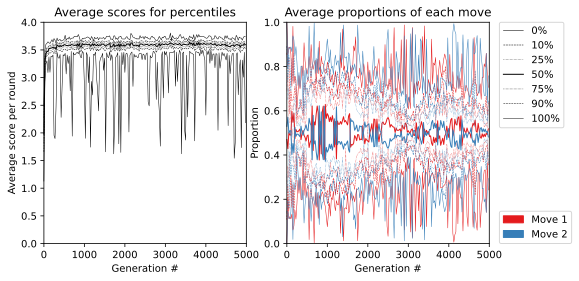
\includegraphics[width=4in]{1607068848885-completed/scores.png}
  \caption{Result graphs from test matrix 1.}
  \label{fig:1607068848885-graphs}
\end{figure}

The example shown above (Figure \ref{fig:1607068848885-graphs}) uses the payout matrix $M=
\begin{bmatrix}
  2 & 1\\
  3 & 0
\end{bmatrix}$ This is similar to the usual \textit{collaborate} vs. \textit{steal} dilemma, where stealing is the dominant strategy, but collaborating networks will out-score networks that always steal. The first graph represents the average score per round for each percentile of players, while the second graph represents a stacked representation of the distribution of each move. Area below the red line (Move 1) represents the proportion of the first move being played, while area above the red line represents the second move. Clearly, the second move is played much more often (around $80\%$ of the time) than the first.

As expected, the average score per round is below $2,$ because networks often fall into a "steal" loop where, much like human players, no mutual trust is formed, and instead both networks continuously steal from one another to prevent losing. However, the relatively high score (though below $2$) is due to a slight change in the matrices: \textit{both stealing} gains both players $0$ points, whereas being \textit{stolen from} (collaborating while opponent steals) incurs a higher payout of $1$ point, eliminating the dominance of stealing as a strategy, and encouraging some collaboration. The lack of significant change in move distribution and scores beyond the first few generations is also notable; it represents the fact that the neural networks reached near a local maximum score-optimizing strategy, one that remained undefeated for the duration of all $5000$ generations.

\begin{figure}[h]
	\[\begin{array}{l r|l}
		&\text{Memory Input} & \text{Move Probabilities} \\
		\hline
		1&{[1, 1, 1, 1, 1, 1]} & {[0.937, 0.063]} \\
		2&{[0, 0, 0, 0, 0, 0]} & {[0.015, 0.985]} \\
		3&{[1, 1, 1, 1, 1, 2]} & {[0.999, 0.001]} \\
		4&{[1, 2, 1, 2, 1, 2]} & {[1.000, 0.000]} \\
		5&{[1, 1, 1, 1, 2, 1]} & {[0.104, 0.896]} \\
		6&{[2, 2, 2, 2, 2, 2]} & {[0.048, 0.952]} \\
	\end{array}\]
  \caption{Test cases for first dataset with memories and probability information.}
  \label{fig:1607068848885-cases}
\end{figure}

This behavior is reflected in the neural networks' actions given certain memory states. In the above graph (Figure \ref{fig:1607068848885-cases}, selected memory states were given to the top-scoring neural network from the last generation ($5000$ in this case), and the move probabilities represents the output layer created by the network, dictating how  likely it wants each move to be played. Notably, due to the smaller size of the payoff matrix, the neural networks only have a length of $3$, where each chunk of $2$ represents the player's move and the move of their opponent, respectively. Of course, the actual memory input would be twice as large, as described in section \ref{subsubsection:NNs}.

This neural network displays a level of intellect un-attainable through simpler strategies in nearly all of these cases. Firstly, in the case with $6$ ones, which represents a situation where for the last $3$ games, both players collaborated, the network acts much like a human player---it continues collaborating, despite theoretically being able to make even more profit from stealing. It is important to note, however, that this happens only $93.7\%$ of the time, showing that the neural network does have a chance, though small, of occasionally stealing.

The third and fourth test cases, however, show a seemingly horrible strategy: continue collaborating if stolen from. Intuitively, one would steal when stolen from, as it prevents the opponent from gaining more points, and decreasing the player's chance of survival. This discrepancy is explained by the second case, which describes a neural network's inital move, given an empty memory (the first round). Unsurprisingly, the network cheats, but as described by the sixth test case, this would result in an infinite loop --- one where both neural nets cheat each other forever, and neither gets points. A dilemma occurs: if both players continue cheating, both will end up with $0$ points, and thus will also have $0$ chance to survive. Once again, the neural network utilizes proportions. The $4.8\%$ chance of collaborating creates a situation where considering each network plays $70$ games of $30$ rounds each, in a majority of these games one network (but rarely both) will cheat, an event which sets off a cheat-collaborate chain, and one player gets $3$ points each while the other gets $1$. This is especially obvious considering the astronomically high proportions for the third and fourth cases, suggesting that the neural network is nearly completely sure it wants to continue the situation, despite it being more advantageous to the opponent. 

Such a strategy will allow neural networks to (ignoring the initial steals) be the stealer half the time, and the collaborator the other half, resulting in an average score of $2,$ equal to that of collaborating. Thus, the networks can use a stealing strategy to eliminate strategies closer to \textit{always collaborate}, while still outdoing strategies such as \textit{always steal} with a cleverly learnt behavior. What is most surprising about this behavior, however, is something that appears many times in later datasets --- neural networks adapt to outplaying simple strategies as expected, but also evolve to collaborate with one another. Such a strategy would be hard-pressed to come across within a purely competitive environment, as no player would want to be the losing one, but often times the neural networks choose a collaborative form of evolution, where networks with similar strategies evolve to work together and keep their "species" dominant, rather than competing simply for self gain.

\subsection{Matching and Mismatching}

TBD.

\section{Discussion}

All in all, the experiments discussed within this paper were a resounding success. Despite initial setbacks regarding network design and processing power constraints, most issues were resolved through redesigning, code optimization, and multithreading over the first few days of experimentation. The neural networks achieved an unexpected level of complexity given their small size, and managed to optimize their strategies far beyond what was initially expected.

Despite the successes of these experiments, however, the project definitely was constrained in a number of ways, most of which can be attributed to the lack of time. Simulations take processing power, and processing time; despite using multithreading and math optimization, 5000 generations often took an average of $12$ hours, given that (on average) each test contained $100$ neural networks, each playing around $60$ games, with $40$ rounds each, adding up to a whopping $240,000$ games per generation, including calculating moves for each player each round, and adding score totals, and eventually selecting survivors and reproducing. Naturally, only a limited number of tests were able to be run, and room for later re-testing was limited. Given more time, larger neural networks could be run containing more nodes and hidden layers, a larger population of networks could be used to allow for greater diversity in strategy, and more games could be played each generation. Furthermore, more complicated payoff matrices could be designed, containing more than four moves and maybe even more than three players. These could be more thoroughly human-tested to compare human strategies with those devised by the networks. Data analysis was similarly restricted; more time could allow for exploration of how neural networks fared against human opponents, observations into how exactly the neural networks managed to devise such complex behavior through analyzing weights, and more. All in all, this project, though successful, can still be taken much further than it was in this short period, and much deeper analysis could be performed on the resultant data.

\end{document}